\documentclass[11pt]{article}
\usepackage[T1]{fontenc}
\usepackage[margin=1.2in,top=0.6in,bottom=0.6in]{geometry}
\usepackage[bookmarks,colorlinks=true,linkcolor=blue,urlcolor=blue]{hyperref}
\usepackage{url}
\usepackage{tabularx}
\usepackage{graphicx}
\usepackage{placeins}
\usepackage{paralist}
\usepackage{makecell}
\usepackage{colortbl}
\usepackage{gensymb}
\usepackage{textcomp}
%\usepackage[osf]{libertine}
\usepackage{zi4}
\usepackage{float}
\usepackage[libertine,cmbraces]{newtxmath}

%\usepackage{draftwatermark}


% table lines
\newcommand{\thinhline}{\Xhline{1\arrayrulewidth}}
\newcommand{\thickhline}{\Xhline{2.5\arrayrulewidth}}
\newcommand{\rtm}{\textsuperscript{\textregistered\space}}

\begin{document}

\title{AKL-PT5 8 GHz Passive Probe Operator Manual}
\author{Antikernel Labs}
\date{\today}

\maketitle
\thispagestyle{empty}

\pagebreak

\tableofcontents

\pagebreak

\section{Overview}

\subsection{Manufacturer}
Antikernel Labs \\
PO Box 4665 \\
10355 NE Valley Rd \\
Rollingbay, WA 98061-0665 \\
\href{https://www.antikernel.net/}{https://www.antikernel.net/} \\
\href{mailto:sales@antikernel.net}{sales@antikernel.net} \\

\subsection{Warranty}

Antikernel Labs warrants this probe to meet published specifications during ordinary laboratory use and operation for a
period of one (1) year from date of shipment and will repair or replace, at its sole option, any defective product.
This warranty covers manufacturing and assembly defects only. Damage caused by negligence, misuse, accident, unapproved
alterations, or exceeding published operating limits is specifically not covered. The tip resistor, ground lead, and
mounting wire are consumable and are expected to degrade over time from repeated soldering, desoldering, and flexing;
damage from ordinary wear and tear is not covered.

Antikernel Labs's maximum liability under this warranty is limited to the replacement value of the probe. Antikernel
Labs will not be liable for any direct, indirect, special, exemplary, or consequential damages (including, but not
limited to, procurement of substitute goods or services, loss of use, data, or profits; or business interruption)
arising in any way out of the use of this probe, even if advised of the possibility of such damage.

\subsection{Open Hardware}

The most up-to-date design files for this probe may be found on GitHub under the 3-clause BSD license, including:

\begin{itemize}
\item KiCAD schematic
\item KiCAD board layout
\item Board fabrication notes including stackup and impedance
\item Sonnet field solver models
\end{itemize}

The current location of design files as of this writing is:
\url{https://www.github.com/azonenberg/starshipraider/}, under the AKL-PT5 subdirectories.

\subsection{Regulatory Compliance}

This probe is RoHS compliant. Exemption 6(c), lead in copper alloys, applies to the brass connector bodies. All other
components of the probe and cable, including solder, are lead free.

\pagebreak
\section{Safety Information}

To avoid personal injury, damage to the probe, or damage to the attached instrument, it is important to understand and
follow the warnings and specification limits in this document.

\begin{itemize}
\item Only personnel familiar with the safe use and operation of electronic test equipment should use this probe.
\item Do not connect the ground terminal of this probe to any voltage other than earth ground.
\item Do not exceed operating limits in the specifications section of this document.
\item The soldermask on this probe is \emph{not} rated for insulation against hazardous voltages, and conductive
elements are exposed at the tip and connector. Do not use this probe on any circuits which may contain voltages
exceeding 30 Vrms, or the touch-safe voltage limit in your organization's standard operating procedures if this is
lower.
\item Do not operate in damp or wet conditions, or under temperature/humidity extremes in which condensation is
likely.
\item Do not operate this probe in a flammable or explosive atmosphere.
\item Wear eye protection and ensure good ventilation when soldering.
\item The SMPM connector center terminal is made from beryllium copper (BeCu) alloy. While exposure to beryllium is
expected to be insignificant during ordinary use of this product as the BeCu is in solid form and covered by gold
plating, hazardous dust could potentially be generated if the contact material is ground or abraded.

CA PROP 65 WARNING: This product can expose you to beryllium, which is known to the State of California to cause cancer.
\end{itemize}

\pagebreak
\section{Theory of Operation}

Tha AKL-PT5 probe is a \emph{transmission line probe} and works very differently from high-impedance passive or active
probes many engineers are familiar with. It is intended primarily for probing relatively low impedance ($50 \Omega$),
high bandwidth digital signals, which ordinarily require expensive active probes to properly examine.

\begin{figure}[h]
\centering
%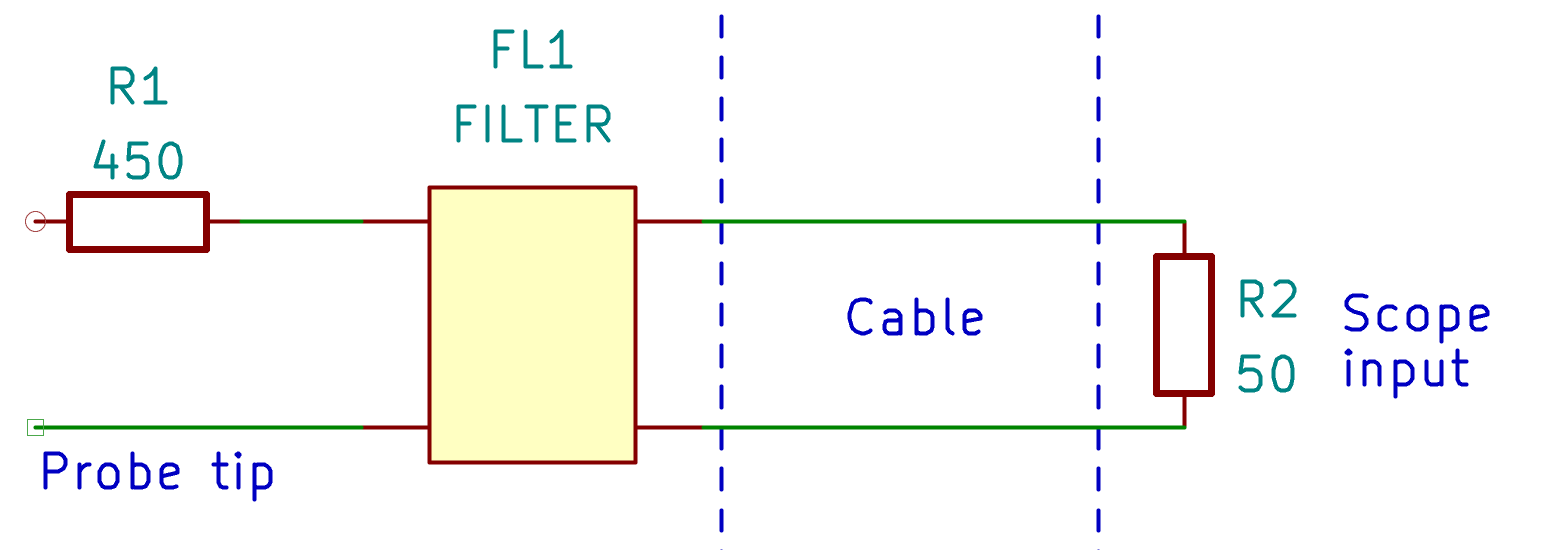
\includegraphics[height=4cm]{schematic.png}
\caption{Simplified probe schematic}
\label{schematic}
\end{figure}

The signal is split off from the DUT at the point of contact and travels through a $450\Omega$ resistor at the
probe tip. It then travels on $50\Omega$ transmission line through a SMPM connector and coaxial cable to the
oscilloscope, which terminates the signal with $50\Omega$ to ground. The tip resistor and termination form a 10:1
voltage divider, so the oscilloscope sees the incident signal attenuated by a factor of 10 (-20 dB). \emph{Note that a
$50 \Omega$ termination at the instrument is required. This probe cannot be used with lower-cost oscilloscopes that
only have $1M \Omega$ terminations.}

The tip resistor and scope-side termination in series present a total loading of $500 \Omega$ on the DUT. While this is
a significantly lower DC impedance than conventional probes, the resistive input stage has extremely flat frequency
characteristics with much less capacitance than conventional passive probes. This means that the impedance of the probe
remains comparatively constant across the entire operating range, rather than greatly decreasing at higher frequencies.

\pagebreak

\section{Usage Instructions}

Proper soldering and desoldering technique is crucial to getting the best performance and lifetime from your probe.

\subsection{Probe Coupling}

Transmission line probes such as the AKL-PT5 have significantly higher DC loading than a standard $10M\Omega$ passive
probe, and may interact poorly with pull-up/pull-down resistors or level shifters with automatic direction sensing.
Consider AC coupling (using an industry standard SMA inner DC block between the probe and coaxial cable), or use of a
different type of probe for these applications.

\subsection{Test Point Design}

The probe tip leads are flexible and can mate with signal and ground contacts at arbitrary spacing from 0 to 8mm. The
natural spacing of signal and ground contacts, requiring the least amount of bending of the leads, is 2.0 mm.

Avoid placing test points in confined spaces between components or in other difficult-to-reach locations. The probe PCB
is nominally 5.6 mm wide so a minimum width of 6.0 mm is suggested for a free fit allowing for PCB routing tolerances.
Sufficient clearance around the signal and ground contacts for hand soldering must be provided, taking into account the
location of the probe PCB itself.

%%%%%%%%%%%%%%%%%%%%%%%%%%%%%%%%%%%%%%%%%%%%%%%%%%%%%%%%%%%%%%%%%%%%%%%%%%%%%%%%%%%%%%%%%%%%%%%%%%%%%%%%%%%%%%%%%%%%%%%%

\subsection{Placing and Securing}

The probe leads are fragile and not intended to be load bearing. When working with any solder-in probe, it is critical
to provide a firm mechanical attachment \emph{before} soldering the tip. Securing a probe operating at microwave
frequencies, such as the AKL-PT5, requires additional care to avoid degrading the performance of the system.

The AKL-PT5 contains an integrated mounting fixture consisting of an 0.5 inch (12.7 mm) square FR4 ``foot" and a FIXME
length of 20 AWG (0.81mm) insulated solid copper wire, attached to each other and the probe head with SAC305 solder.
The mounting wire is considered to be a consumable and is expected to eventually fail from repeated bending over the
lifetime of the probe. The mounting wire may be easily replaced with a new piece of wire\footnote{While the supplied
mounting wire was chosen to provide a reasonable default for most applications, feel free to customize your probe by
replacing it with a longer, shorter, stiffer, or more flexible wire if your application dictates.} by hand soldering
when this happens.

Determine which side of the test point you intend for the probe to approach from and ensure a good ground point is
easily reachable. If your probe is configured with the ground lead on the wrong side\footnote{For convenience, the
AKL-PT5 is available with one of two ground lead placements from the factory, to the left (AKL-PT5L) or right
(AKL-PT5R) of the signal contact as seen with the SMPM connector facing upward. The PCB is identical for both variants,
and the ground lead can be easily swapped from one footprint to the other in the field with a soldering iron.} of the
signal contact, desolder it and reattach it to the opposite footprint.

To mount the probe, begin by selecting a suitable location for the mounting foot, typically about 1 inch (25 mm) from
the test point. Hold the foot in place and pre-bend the mounting wire to place the probe head close to the test point
to check the fit.

Once you are satisfied with the placement, if the probe head and cable are not already attached, connect the SMPM cable
to the probe head by grasping the cable connector and probe PCB firmly with two fingers and pressing the connectors
straight into each other. You may hear or feel a slight click when the connector seats fully, but this may not be
noticeable.

DO NOT attempt to mate or unmate the SMPM connector once the probe is soldered to the DUT. This may result in damage to
the test point, probe, or both. Always mate the connector prior to soldering, and desolder the probe prior to unmating.

Select a piece of double-sided tape and attach one side of the tape to the underside of the mounting foot. The AKL-PT5
ships with sample quantities of two different types of tape: a clear rubbery material and a white polyurethane foam.
For information on ordering additional tape, see the Ordering Information section.

Both tapes may be removed from the probe and DUT without damage or leaving residue, however the white foam tape
provides significantly greater holding force when attached to typical PCB materials. It is typically used for longer
term, semi-permanent measurements; the clear tape has a weaker adhesive and may be preferable for shorter term use when
the probe is expected to be frequently repositioned.

Remove the liner from the tape and secure the foot to the desired location.

\begin{figure}[h]
\centering
%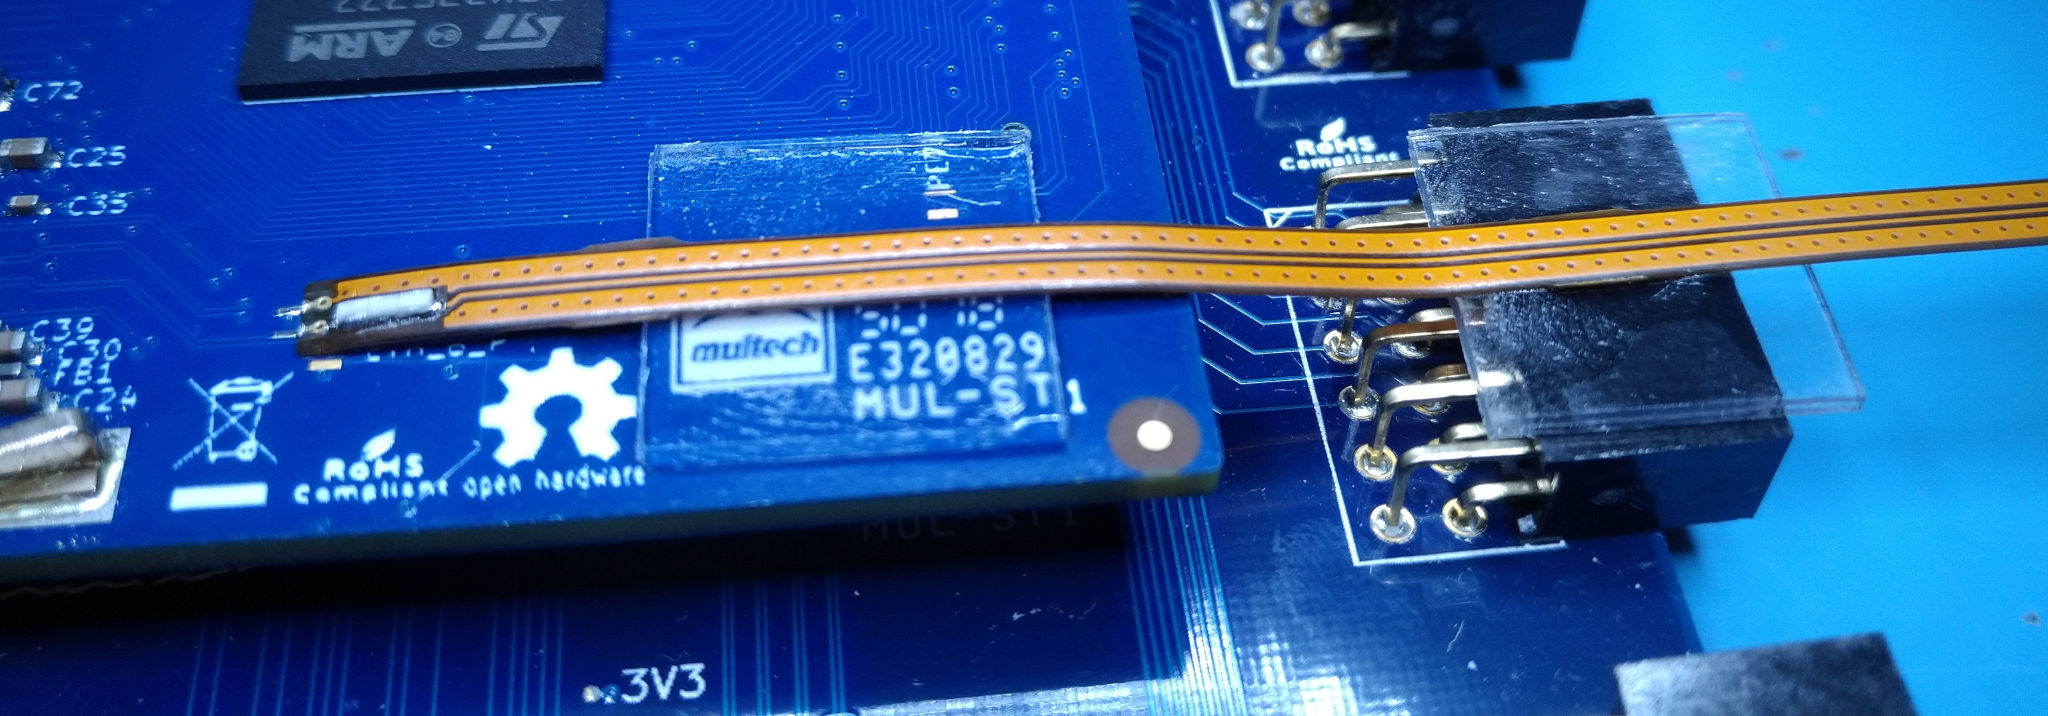
\includegraphics[width=12cm]{secured-tip.jpg}
\caption{AKL-PT5 probe mounted to DUT with double-sided adhesive squares}
\label{secured-tip}
\end{figure}

The coaxial cable attached to the probe should also be secured to prevent applying excessive force to the probe body,
as the mounting wire is too flexible to resist a significant tug on the cable without the probe head moving. Any method
providing adequate mechanical support may be used; an example setup using polyimide tape is shown in Fig.
\ref{cable-secured}. Leave a small amount of slack at the probe end of the cable so that the probe head can move
slightly during soldering.

\begin{figure}[h]
\centering
%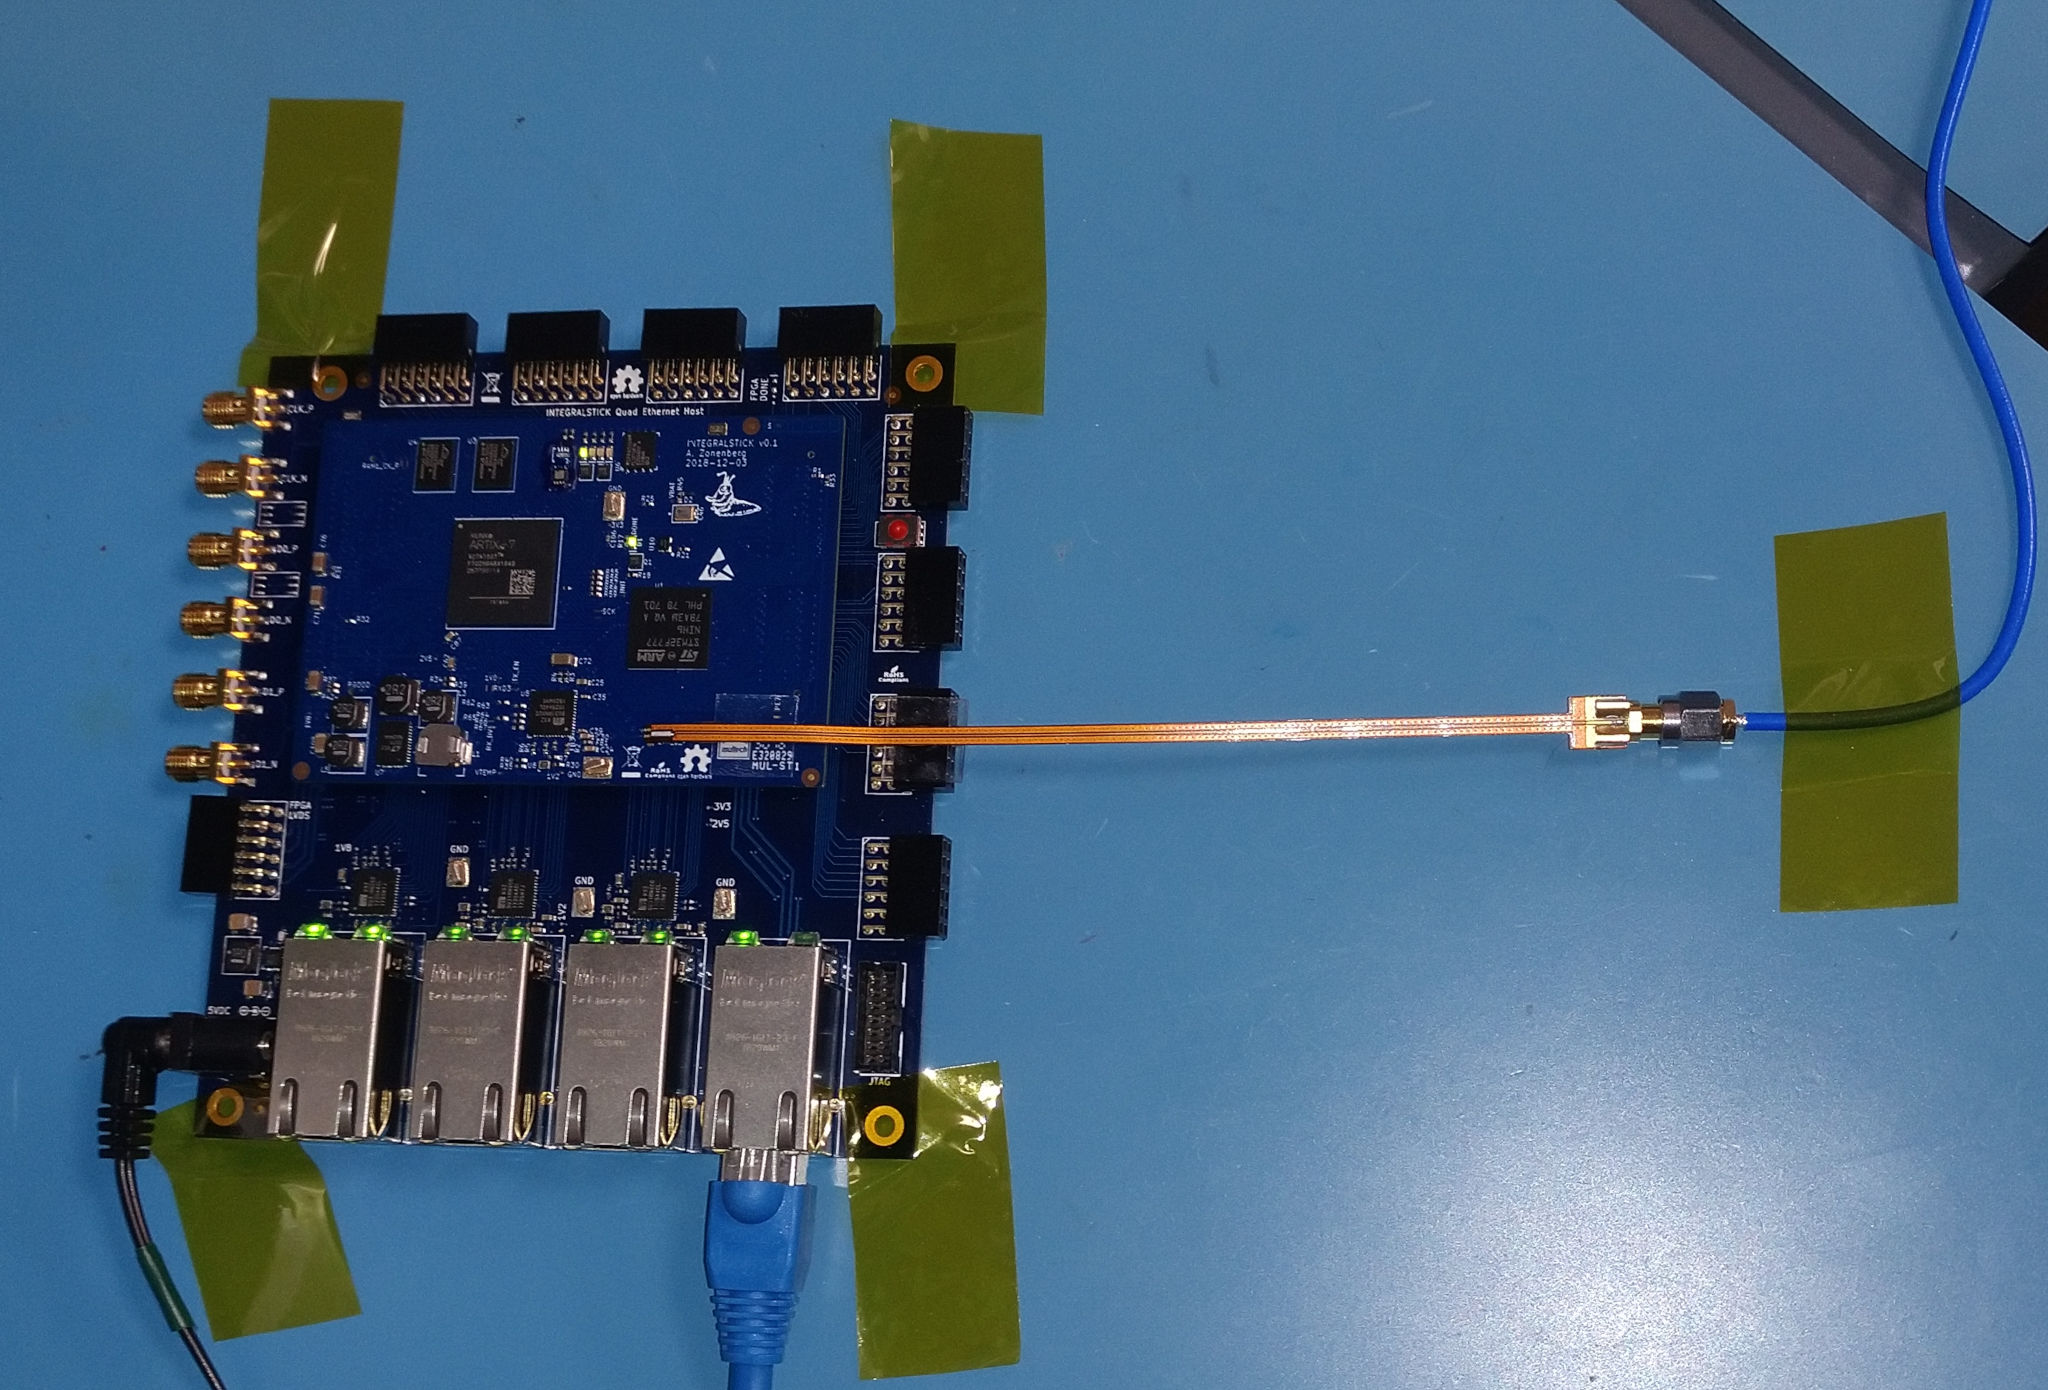
\includegraphics[width=12cm]{cable-secured.jpg}
\caption{Securing cable and DUT to lab bench with polyimide tape}
\label{cable-secured}
\end{figure}

\FloatBarrier

\subsection{Soldering}

Once the mounting foot is secured to the DUT and the mounting wire is bent correctly, the head should be floating just
above (typically about 1mm) the test point. Use tweezers to pre-bend the signal and ground leads so that the tips are
correctly spaced for your test points. The probe body should be roughly centered between the signal and ground points
so that both leads bend approximately the same amount. The goal is for the springiness of the mounting wire to hold the
leads under very slight tension once soldered - just enough to keep them taut, but not enough to place significant
force on the solder joints.

Remove soldermask from the signal and ground test points with a scraper if necessary, and tin the points with a fine
point soldering iron.

Apply a small amount of flux to the ground test point. Grasp the probe body with one hand while holding the soldering
iron in the other. Gently move the probe body to press the ground lead against the tinned test point, then melt the
solder to form the joint. Ensure the solder solidifies fully before letting go of the probe. (Soldering the ground
point before the signal point helps reduce mechanical stresses on the DUT signal traces, which are typically smaller
and less mechanically robust than large ground planes or bypass capacitor pads.)

Apply flux to the signal test point, then use tweezers to position the signal lead against the tinned test point and
solder it. Inspect the joints as necessary. For best accuracy and lowest loading, remove flux from the probe tip area
after soldering using isopropyl alcohol on a lint-free swab.

\begin{figure}[h]
\centering
%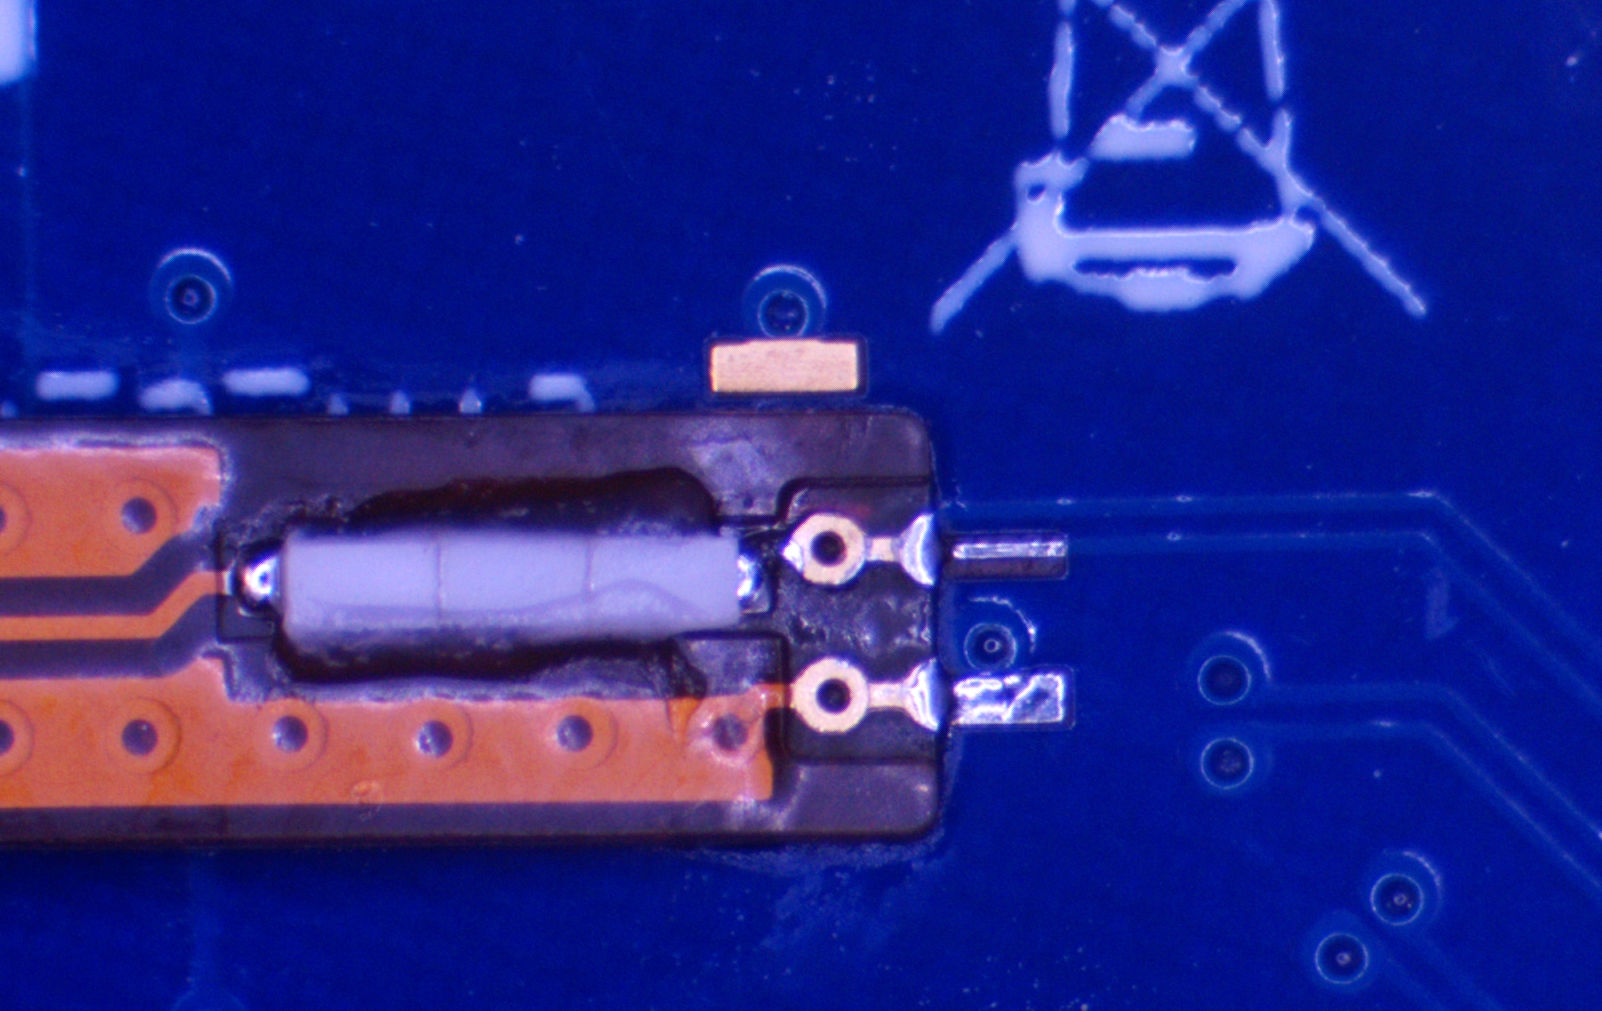
\includegraphics[width=8cm]{tip-on-testpoint.jpg}
\caption{AKL-PT5 tip soldered to test point}
\label{tip-on-testpoint}
\end{figure}
\FloatBarrier

\subsection{Desoldering}

Use a soldering iron to melt the solder on the signal contact, then gently nudge the probe tip wire to one side with
tweezers. Desolder the ground lead after the signal lead is free of the DUT, holding the probe body or mounting wire
with your other hand to prevent it from moving suddenly as the solder melts.

Remove any excess solder from the tip leads and test points with desoldering braid.

After desoldering is complete, gently peel the mounting foot off the DUT and discard the used adhesive pad. The clear
tape's adhesive has a lower peel strength and should not require any special techniques to remove; the white tape is
significantly stronger and requires more effort to remove. It may be necessary to apply some prying force at a corner
of the foot-to-tape joint with a spudger or similar tool. Once the probe is free of the tape, the tape on the DUT
should come free easily by peeling from one corner, without leaving behind any residue on the probe or DUT.

To unmate the cable from the probe, grasp the probe head by the edges between two fingers with one hand while holding
the SMPM connector of the cable between two fingers of the other hand and pull them apart with a slight rocking motion.
Do not apply any force to the coaxial cable or heat shrink tubing as these are not designed to handle significant
tensile loads. You may be able to get a better grip on the cable connector by using your fingernails to pull the front
face of the connector away from the probe (Fig. X)

\subsection{Maintenance, Cleaning, and Storage}

To avoid attracting dust or corroding the tip contacts, when the probe is being stored it is best to remove flux
residue from the tip area. This may be done with isopropyl alcohol and a lint-free swab, or any other industry-standard
flux remover suitable for the flux in question.

The SMA connector on the supplied cable is gaged before shipment to ensure the pin and dielectric position are within
tolerance, however it is good practice to gage the connector periodically to detect any gradual misalignments as the
connector wears.

No other maintenance is normally required.

The probe should be stored in the provided foam-lined cardboard box when not in use to protect the fragile tip contacts
from mechanical damage. The foam and cardboard are static dissipative to ensure ESD safety and prevent charges from
building up on the probe which could damage surrounding equipment, however the probe itself has no active components
and does not require special handling for ESD reasons.

\FloatBarrier
\subsection{Cables}

The AKL-PT5 must be connected to the host instrument via a $50 \Omega$ coaxial cable with low loss over the operating
bandwidth of the probe, terminated with a SMPM female connector at the probe side. The stock cable supplied with the
probe is Koaxis part number AO10-KF047-RO10-36.00-MC-TD.

The cable should be taped to a lab bench or the DUT as shown in Fig. \ref{cable-secured}, or otherwise secured to
prevent transferring any force into the probe.

%%%%%%%%%%%%%%%%%%%%%%%%%%%%%%%%%%%%%%%%%%%%%%%%%%%%%%%%%%%%%%%%%%%%%%%%%%%%%%%%%%%%%%%%%%%%%%%%%%%%%%%%%%%%%%%%%%%%%%%%

\pagebreak
\section{Mechanical Specifications}

\begin{tabularx}{10cm}{Xrr}
\thickhline
\textbf{Description} & \textbf{Typ} & \textbf{Units} \\
\thickhline
Mass (probe head and mounting foot) & xx & g\\
\thinhline
Height (probe head) & xx & mm\\
\thinhline
Length (probe head PCB) & 10.2 & mm\\
\thinhline
Length (probe head and tip resistor) & xx & mm\\
\thinhline
Width & 5.3 & mm\\
\thickhline
\end{tabularx}

\pagebreak
\section{Electrical Specifications}

Values in this section are typical / limit values. For measured values from a specific probe, please consult your
calibration certificate.

\subsection{Absolute Maximum Ratings}

Exceeding these limits may result in permanent damage to the probe. Ratings in this section are stress ratings only and
normal operation at these limits is not implied.

\begin{tabularx}{12cm}{lXrl}
\thickhline
\textbf{Parameter} & \textbf{Description} & \textbf{Limit} & \textbf{Units} \\
\thickhline
$T_{amin}$ & Minimum temperature & 0 & $ \degree C$ \\
\thinhline
$T_{amax}$ & Maximum temperature & 95 & $ \degree C$ \\
\thinhline
$I_{max}$ & Maximum sustained current & xx & $ mA $ \\
\thinhline
$V_{maxT}$ & Maximum sustained tip voltage & xx & $ Vrms $ \\
\thinhline
$V_{maxV}$ & Maximum instantaneous tip voltage & xx & $ Vrms $ \\
\thickhline
\end{tabularx}

ENGINEERING NOTE: The sustained current/voltage limits are thermally limited and based on the 50 mW power rating of the
$200 \Omega$ tip resistors. Brief pulses or low duty cycle waveforms whose average power does not exceed these limits
\emph{may} be possible to probe safely with the AKL-PT5 as long as tip voltage does not exceed the instantaneous
voltage limit at any time, however Antikernel Labs has not performed any testing of the probe under pulsed load
conditions. Use of the probe with instantaneous power levels exceeding the thermal limits will void the warranty and
customer assumes all risk of harm to personnel and equipment resulting from such usage.

%%%%%%%%%%%%%%%%%%%%%%%%%%%%%%%%%%%%%%%%%%%%%%%%%%%%%%%%%%%%%%%%%%%%%%%%%%%%%%%%%%%%%%%%%%%%%%%%%%%%%%%%%%%%%%%%%%%%%%%%

\subsection{Recommended Operating Conditions}

While the probe will not be damaged by exposure to conditions outside the values in this section (but below the
``Absolute Maximum Ratings" limits), tolerances may be temporarily exceeded.

\begin{tabularx}{12cm}{lXll}
\thickhline
\textbf{Parameter} & \textbf{Description} & \textbf{Limit} & \textbf{Units} \\
\thickhline
$T_{min}$ & Minimum temperature & 15 & \degree C \\
\thinhline
$T_{max}$ & Maximum temperature & 45 & \degree C \\
\thinhline
\thickhline
\end{tabularx}

%%%%%%%%%%%%%%%%%%%%%%%%%%%%%%%%%%%%%%%%%%%%%%%%%%%%%%%%%%%%%%%%%%%%%%%%%%%%%%%%%%%%%%%%%%%%%%%%%%%%%%%%%%%%%%%%%%%%%%%%

\subsection{DC Characteristics}

\begin{tabularx}{16cm}{lXrrrr}
\thickhline
\textbf{Parameter} & \textbf{Description} & \textbf{Min} & \textbf{Typ} & \textbf{Max} & \textbf{Units} \\
\thickhline
$G_{dc}$ & Gain across $50\Omega$ load\footnote{Assuming ideal $50 \Omega$ termination at instrument} &  & 0.094 &  & V/V \\
\thinhline
$R_{gnd}$ & Signal path resistance from SMPM to tip & xx & xx & xx & $\Omega$ \\
\thinhline
$R_{sig}$ & Ground path resistance from SMPM tip & xx & xx & xx & $\Omega$ \\
\thinhline
$TCR$ & Temperature coefficient of resistance & & & $\pm 100$ & ppm / \degree C \\
\thickhline
\end{tabularx}

%%%%%%%%%%%%%%%%%%%%%%%%%%%%%%%%%%%%%%%%%%%%%%%%%%%%%%%%%%%%%%%%%%%%%%%%%%%%%%%%%%%%%%%%%%%%%%%%%%%%%%%%%%%%%%%%%%%%%%%%

\pagebreak
\subsection{AC Characteristics}

Data in this section is based on characterization in a $50 \Omega$ environment, with cable and fixture effects
de-embedded, unless otherwise stated.

\begin{tabularx}{16cm}{lXrrrr}
\thickhline
\textbf{Parameter} & \textbf{Description} & \textbf{Min} & \textbf{Typ} & \textbf{Max} & \textbf{Units} \\
\thickhline
$S_{11o}$ & $S_{11}$ across open circuit from DC - 6 GHz & xx & xx & xx & dB \\
\thinhline
$S_{21}$ & $S_{21}$ from DC - 6 GHz & xx & xx & xx & dB \\
\thinhline
$BW$ & -3 dB bandwidth & 8.0 & 8.5 & & GHz \\
\thinhline
$BW_{nodbed}$ & -3 dB bandwidth including cable losses &  & 4 & & GHz \\
\thinhline
$Rise_{90}$ & Rise time (10-90 \%) &  & xx & xx & ps \\
\thinhline
$Rise_{80}$ & Rise time (20-80 \%) &  & xx & xx & ps \\
\thinhline
$Tpd$ & Propagation delay &  & xx &  & ps \\
\thickhline
\end{tabularx}

\pagebreak
\section{Performance Graphs}

\subsection{Insertion Loss}

\begin{figure}[h!]
\centering
%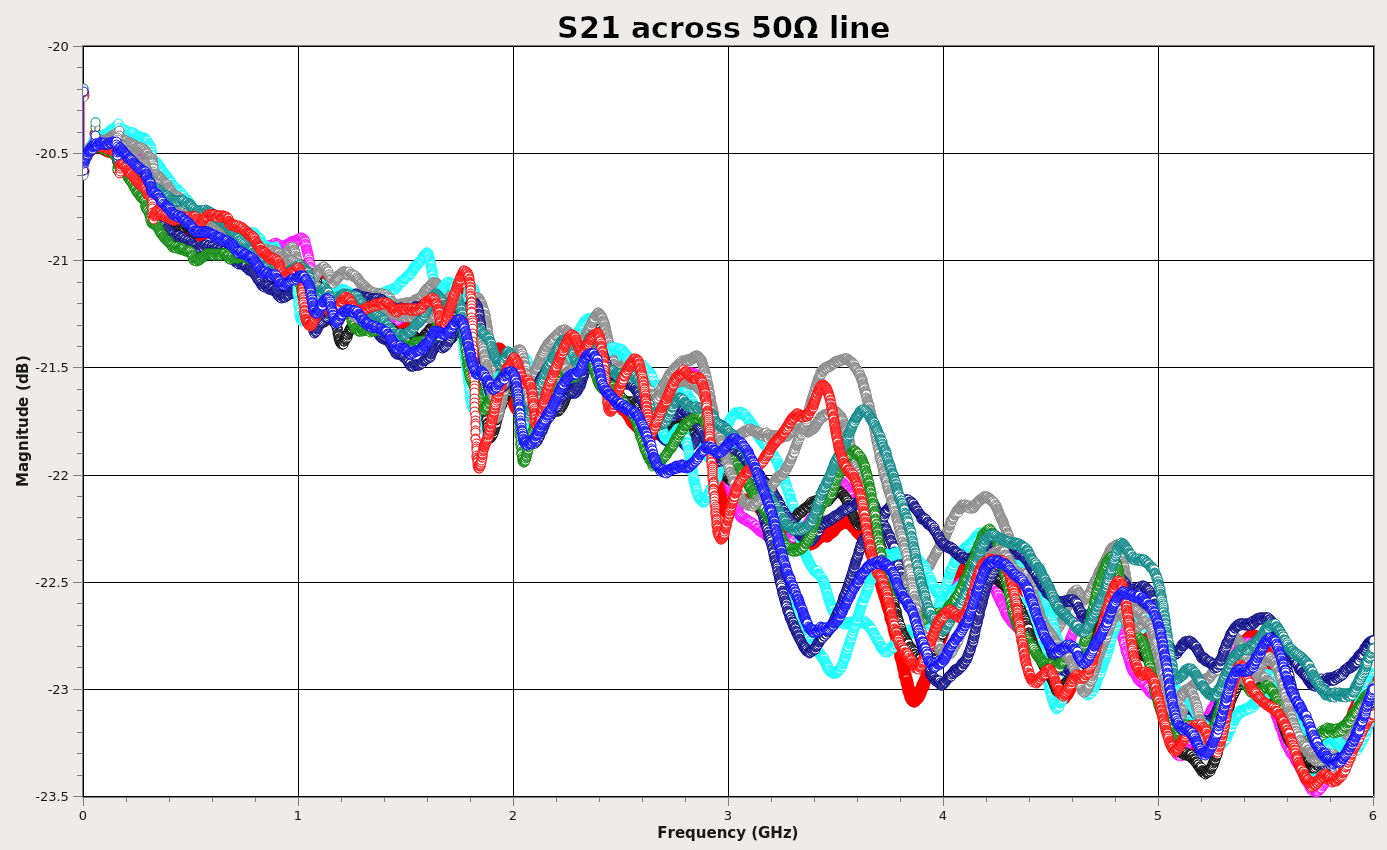
\includegraphics[width=14cm]{s21-variation.png}
\caption{$S_{21}$ range of probes across $50\Omega$ termination}
\label{s21-variation}
\end{figure}

\subsection{Group Delay}

\begin{figure}[h]
\centering
%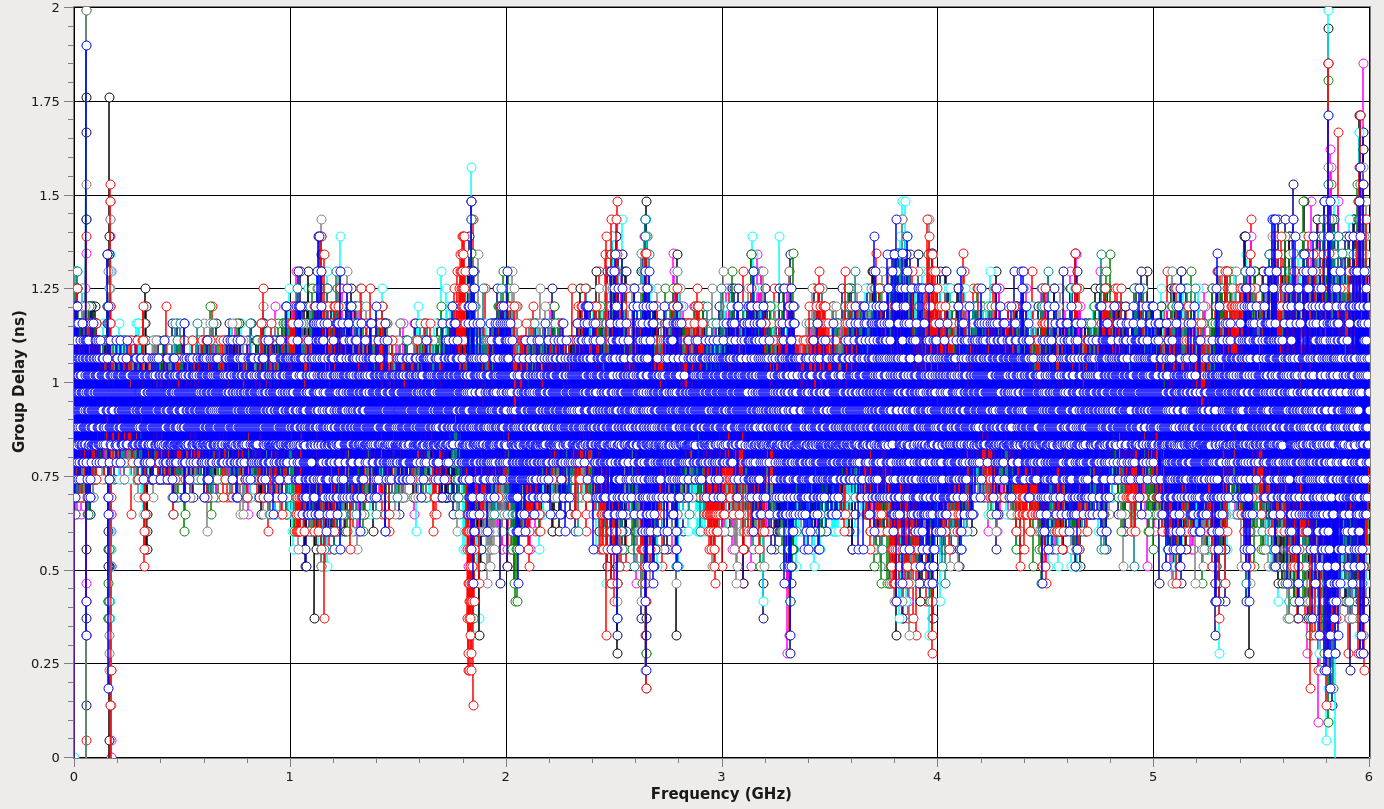
\includegraphics[width=14cm]{groupdelay-variation.png}
\caption{Group delay variation of probes}
\label{typical-groupdelay}
\end{figure}
\FloatBarrier

\pagebreak
\subsection{Return Loss}

\begin{figure}[h!]
\centering
%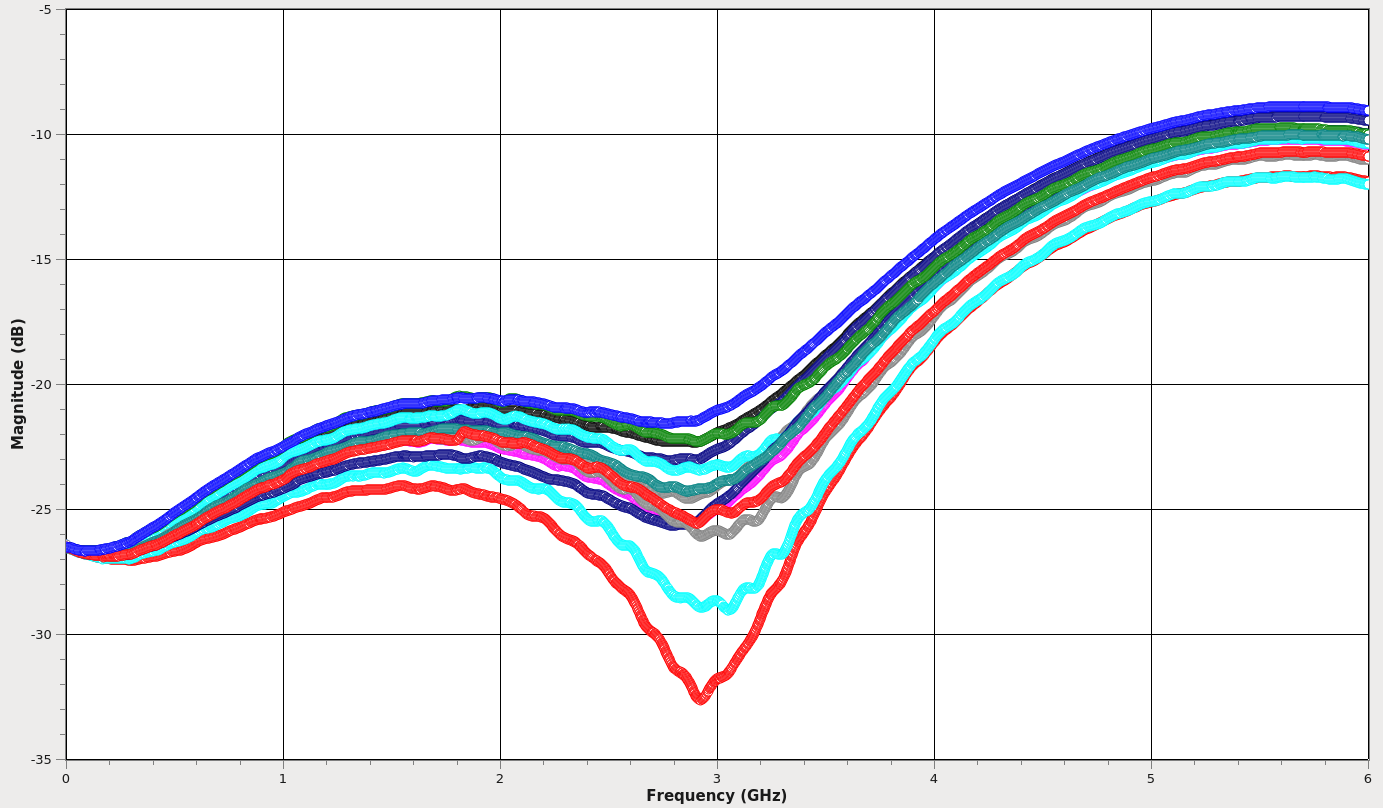
\includegraphics[width=14cm]{s11-variation.png}
\caption{Variation in $S_{11}$ of probes across $50\Omega$ load}
\label{s11-open-variation}
\end{figure}

\begin{figure}[h!]
\centering
%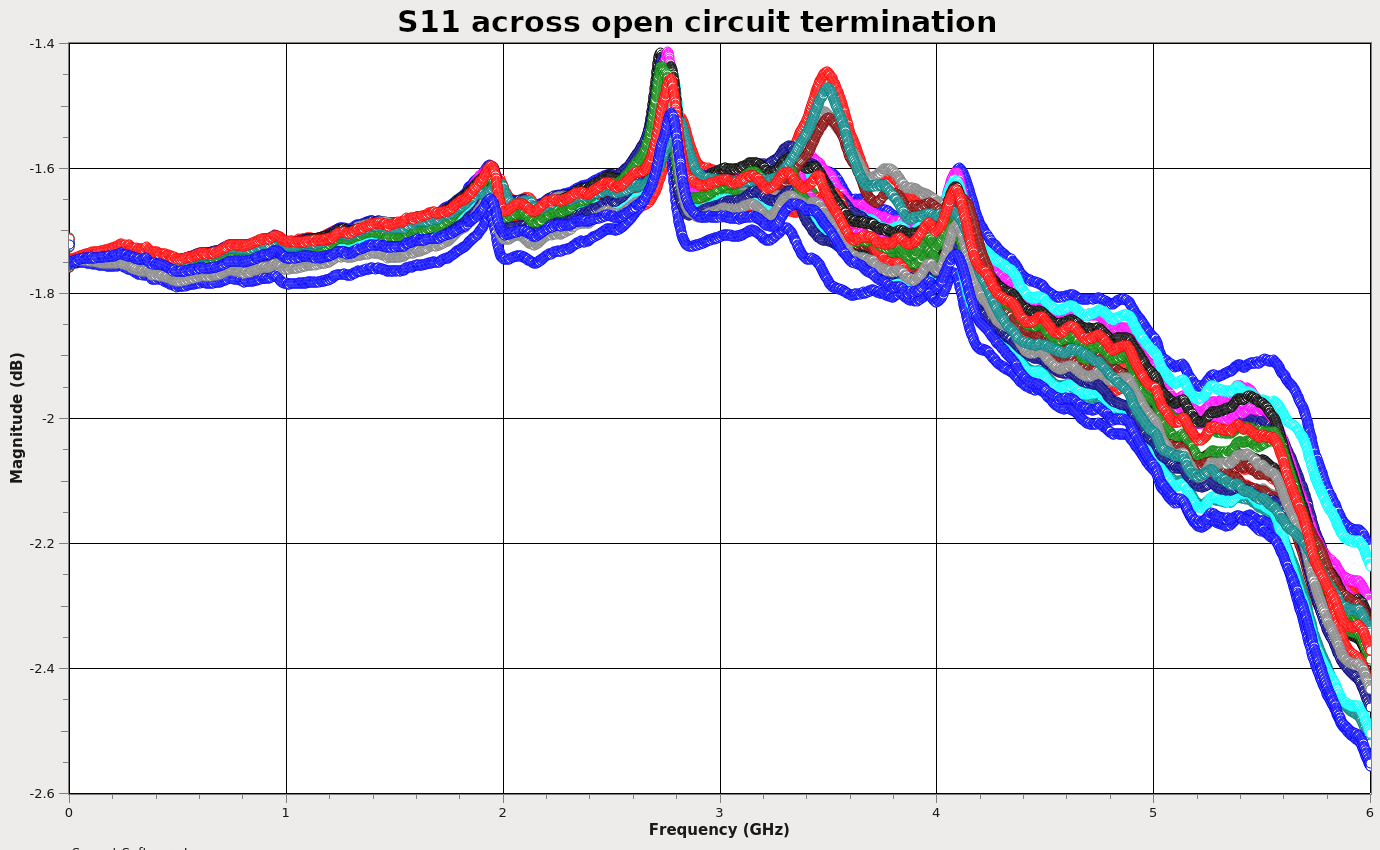
\includegraphics[width=14cm]{s11-open-variation.png}
\caption{Variation in $S_{11}$ of probes across open circuit}
\label{s11-variation}
\end{figure}

\FloatBarrier

\pagebreak
\subsection{Step Response}

\begin{figure}[h!]
\centering
%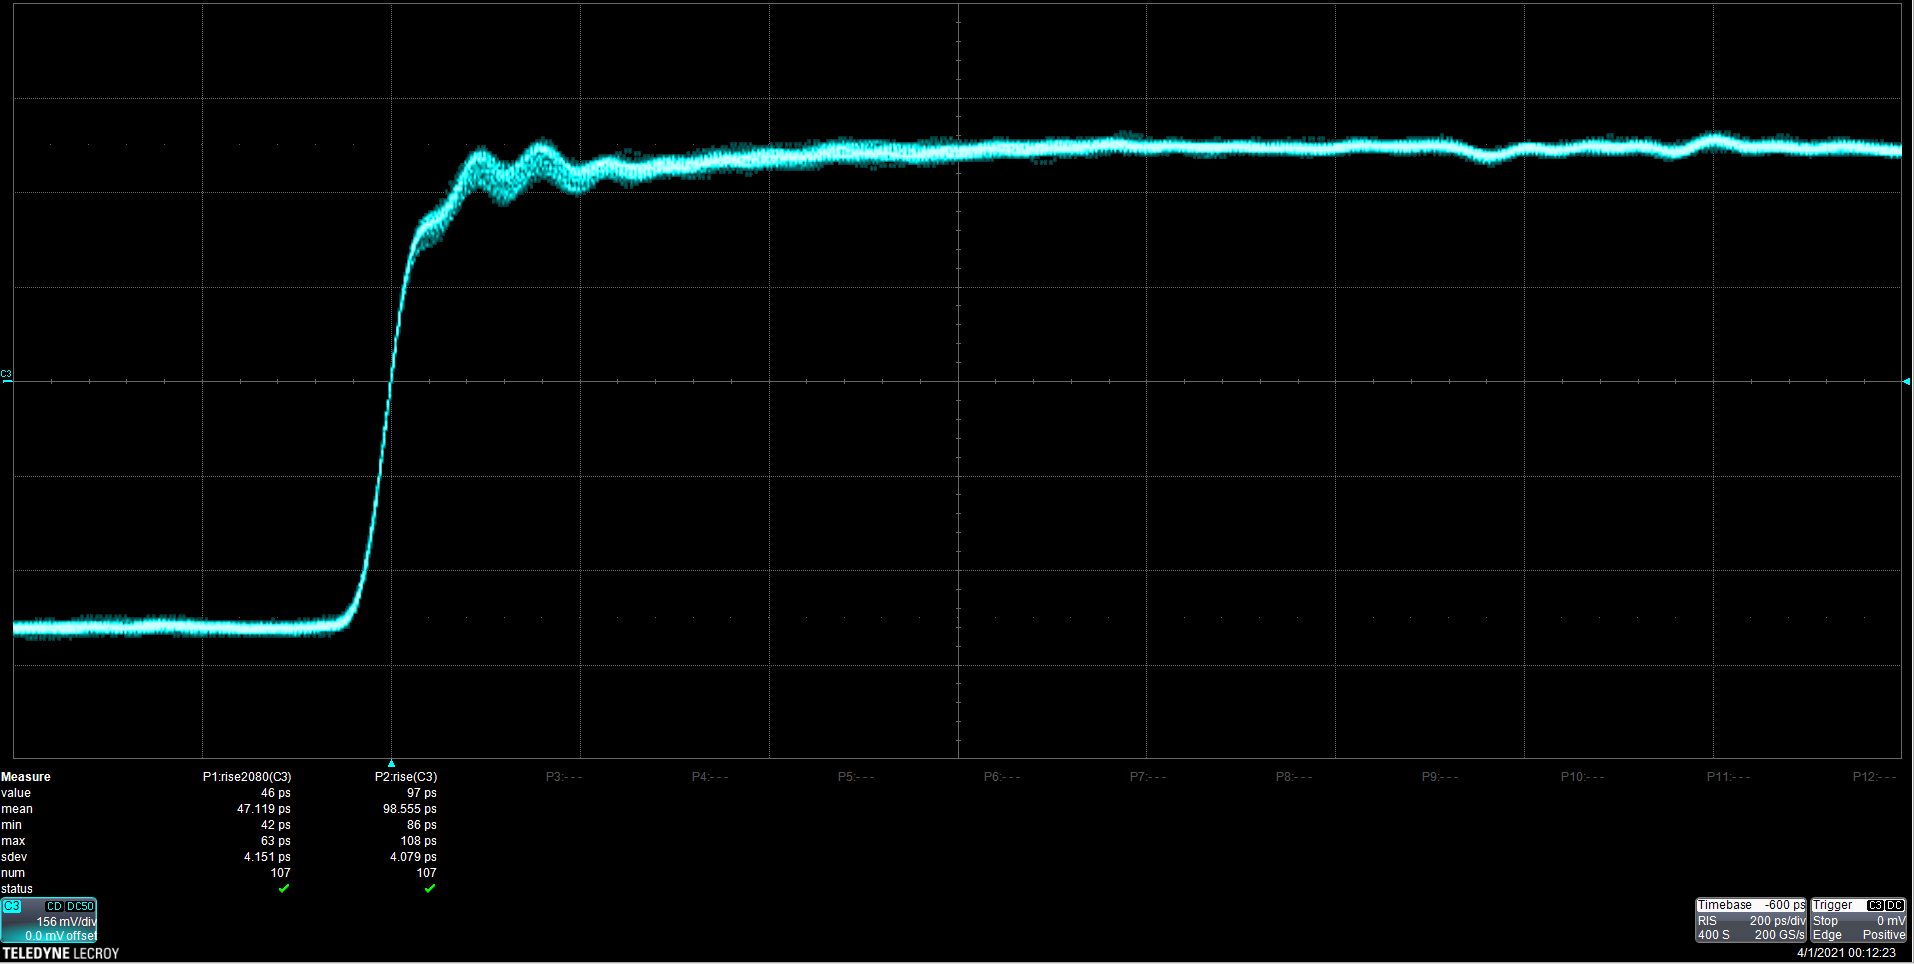
\includegraphics[width=14cm]{step-response.png}
\caption{Typical response of AKL-PT5 to fast rising edge (200ps/div)}
\label{step-response}
\end{figure}

\FloatBarrier

\pagebreak
\section{Performance Data}

If you requested full characterization at the time of your order, test measurements are available at
\url{https://www.antikernel.net/downloads/AKL-PT5/caldata/} and searching for your probe's serial number. All
measurements are de-embedded to the SMPM connector or probe tip, as applicable.

The following S-parameter data files are provided:
\begin{itemize}
\item probe.s2p - probe across $50 \Omega$ load with cable de-embedded
\item cable.s2p - the provided cable
\item system.s2p - probe across $50 \Omega$ load including cable effects
\end{itemize}

Touchstone port 1 is connected to the DUT side of the probe and port 2 (if applicable) is connected to the instrument
side.

%%%%%%%%%%%%%%%%%%%%%%%%%%%%%%%%%%%%%%%%%%%%%%%%%%%%%%%%%%%%%%%%%%%%%%%%%%%%%%%%%%%%%%%%%%%%%%%%%%%%%%%%%%%%%%%%%%%%%%%%

\pagebreak
\section{Ordering Information}

\subsection{Probe}

The standard AKL-PT5 kit includes the probe head, mounting foot, serialized SMA to SMPM cable with S-parameters, and a
starter pack of double-sided mounting tape.

Probe heads may also be purchased with no accessories (other than the mounting foot) for use with existing cables.

\begin{tabularx}{16cm}{llX}
\thickhline
\textbf{Item} & \textbf{Supplier} & \textbf{Part number} \\
\thickhline
Probe kit, left hand ground & Antikernel Labs & AKL-PT5L-KIT \\
\thinhline
Probe kit, right hand ground & Antikernel Labs & AKL-PT5R-KIT \\
\thinhline
Probe head only, left hand ground & Antikernel Labs & AKL-PT5L-HEAD \\
\thinhline
Probe head only, right hand ground & Antikernel Labs & AKL-PT5R-HEAD \\
\thickhline
\end{tabularx}

\subsection{Cable}

The cable supplied in the AKL-PT5 accessory kit is 36 inches in length, SMA straight plug (m) to SMPM straight plug
(f), and made from Koaxis KF047 0.047" coaxial cable. Cables are individually serialized and include S-parameters to
26.5 GHz.

For specialized applications, cables of other lengths or with different scope-side connectors may be ordered directly
from Koaxis. Antikernel Labs recommends using only KF047 cable or equivalent highly flexible micro coax with the
AKL-PT5 to avoid placing excessive mechanical forces on the probe head or solder joints.

\begin{tabularx}{16cm}{llX}
\thickhline
\textbf{Item} & \textbf{Supplier} & \textbf{Part number} \\
\thickhline
Standard cable & Koaxis & AO10-KF047-RO10-36.00-MC-TD \\
\thickhline
\end{tabularx}

\subsection{Consumables}

\begin{tabularx}{16cm}{llX}
\thickhline
\textbf{Item} & \textbf{Supplier} & \textbf{Part number} \\
\thickhline
Mounting tape, clear rubber & Scotch & MMR103B \\
\thinhline
Mounting tape, white polyurethane foam & McMaster-Carr & 76535A21 \\
\thinhline
Mounting wire (25 ft spool) & Remington Industries & 20UL1007SLDBLA25 \\
\thinhline
Tip resistor \footnote{Vishay Dale part number HML01450RFKE05, trimmed to 7.5 mm overall length by Antikernel Labs}
	& Antikernel Labs & AKL-PT5-RESISTOR \\
\thinhline
Ground lead \footnote{0.188 mm (approximately 33 AWG) x 7.5mm tin-plated nickel wire} & Antikernel Labs & AKL-PT5-GROUND \\
\thickhline
\end{tabularx}


\end{document}
